\documentclass{article}
\usepackage{graphicx} % Required for inserting images
\usepackage[a4paper,
             bindingoffset=0.2in,
             left=1in,
             right=1in,
             top=1in,
             bottom=1in,
             footskip=.25in]{geometry}
\usepackage[colorlinks=true,allcolors=blue]{hyperref}
\usepackage{amsmath}
\usepackage[english,nameinlink]{cleveref}
\usepackage{natbib}
\usepackage{url}
\usepackage{subfigure}
\usepackage{setspace}
\usepackage{booktabs}
\usepackage{siunitx}

\title{High Performance Computing final project\\Exercise 1}
\author{Giulio Fantuzzi}
\date{22th February 2024}

\begin{document}

\maketitle
%\tableofcontents
\setstretch{1.15}
\section{Problem statement}\label{section:problemstatement}
This project aims to assess the performance of various \texttt{openMPI} \cite{openMPI} algorithms for specific collective operations, specifically broadcast and barrier. Our objective is to estimate the latency of the default implementation and compare it with values obtained through the selection of different algorithms.

\section{Methodology}\label{section:methodology}
To estimate the latency of the operations, we referred to the \texttt{OSU} benchmark\cite{osu-microbenchmarks}, running its scripts on two \textit{thin}
%---footnote
\footnote{Opting for \textit{thin} nodes in the measurements was driven by the intense activity and prolonged resource allocation times observed on \textit{Epyc} nodes during the data collection phase. Nevertheless, performing experiments on \textit{Epyc} nodes would probably result in similar interpretations, though some adjustments may be needed due to differences in the nodes' structure.}
%---
nodes of the \texttt{ORFEO} \cite{orfeo} cluster. To enhance the efficiency of the analysis, the entire data gathering process was automated by using some bash scripts, which were then submitted to the cluster using the \texttt{SLURM} workload manager, utilizing the \texttt{sbatch} command for streamlined execution. The analyzed problem presented several degrees of freedom, so we got different measures of the latency by varying the number of processes, their allocation and the size of the messages exchanged. We concluded our analysis by attempting to construct a performance model and to extrapolate results basing on the specific architecture on which the operations were executed. For more information about the scripts, check the repository \href{https://github.com/giuliofantuzzi/HPC_FinalProject}{https://github.com/giuliofantuzzi/HPC\_FinalProject}.

\section{Broadcast}\label{section:broadcast}
\subsection{Broadcast algorithms}\label{subsection:broadcast_algorithms}
In addition to evaluating the default \texttt{openMPI} algorithm for broadcast operations, this study incorporates a comprehensive analysis of three alternative algorithms: linear/flat tree (\Cref{fig:linear_algorithm}), chain (\Cref{fig:chain_algorithm}), and binary tree(\Cref{fig:binary_tree_algorithm} ).
\begin{figure}[htp]
    \centering
    \subfigure[Linear algorithm]{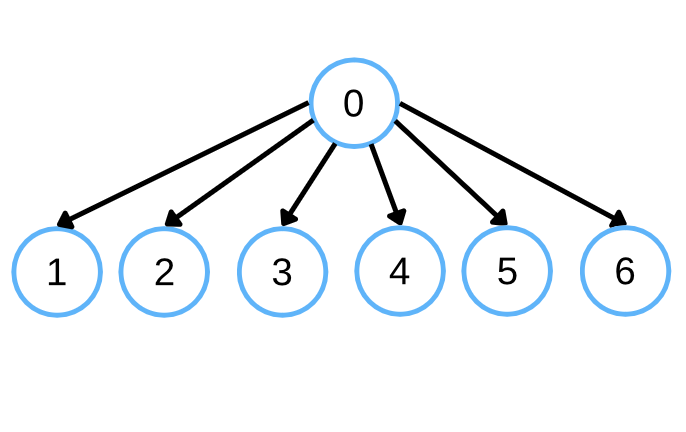
\includegraphics[width=0.3\textwidth]{images/bcast_linear_alg.png}\label{fig:linear_algorithm}}
    \hfill
    \subfigure[Chain algorithm]{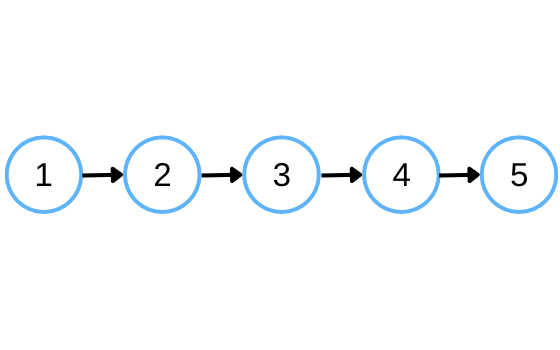
\includegraphics[width=0.3\textwidth]{images/bcast_chain_alg.png}\label{fig:chain_algorithm}}
    \hfill
    \subfigure[Binary Tree algorithm]{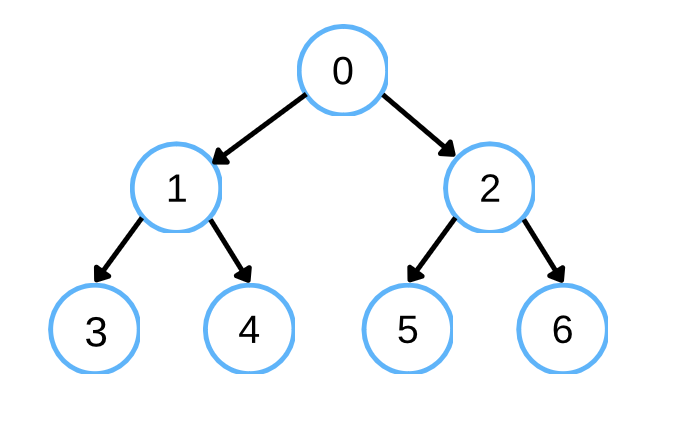
\includegraphics[width=0.3\textwidth]{images/bcast_binarytree_alg.png}\label{fig:binary_tree_algorithm}}
    \caption{\footnotesize Analyzed broadcast algorithms}
\end{figure}

\subsection{Broadcast latency analyses}\label{subsection:broadcast_latency}
The data collection phase generated a sizable dataset, providing latency details for different combinations of algorithm, number of processes, processes allocation and message size. The extensive nature of the dataset introduced a multitude of degrees of freedom, offering flexibility for analysis. To handle this complexity, we initially performed analyses by constraining specific degrees of freedom and emphasizing marginal effects. Subsequently, a thorough examination was carried out to explore the interactions between variables in various ways.
\subsubsection{Fixing algorithm and compare processes allocation effects}\label{subsubsection:map}
For each algorithm, we assessed the influence of process allocation on the operation latency. To maintain the independence of our analysis from message size, we fixed it to 1 \texttt{MPI\_CHAR}, effectively isolating and examining a form of `pure' latency associated with the algorithms.

\begin{figure}[htp]
    \centering
    \subfigure[Linear algorithm]{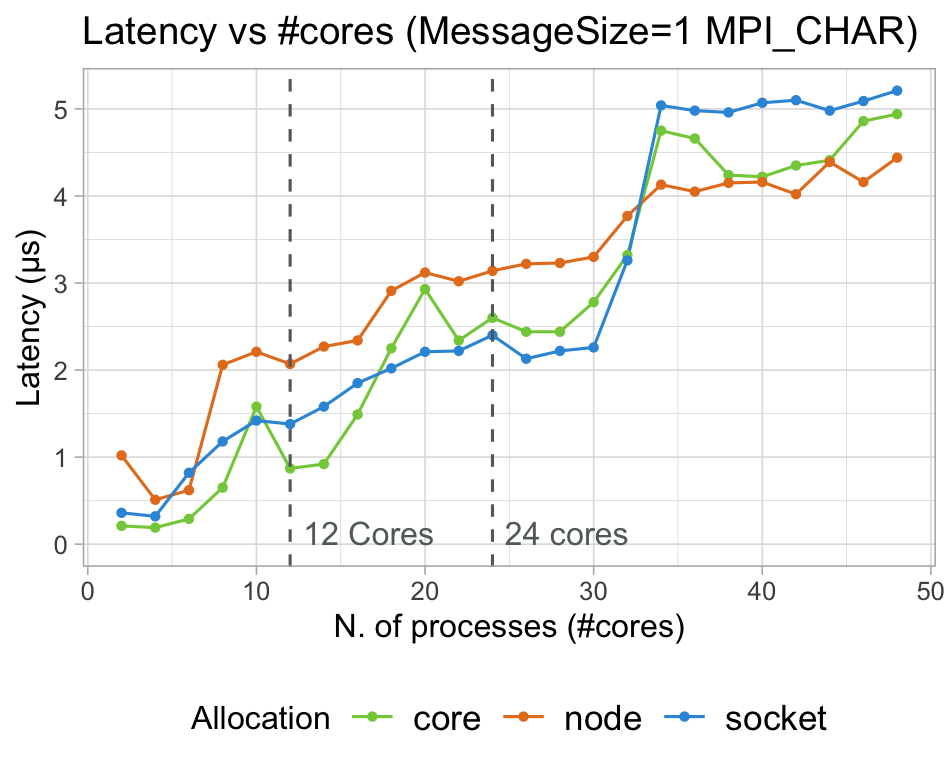
\includegraphics[width=0.32\textwidth]{plots/linear_map.png}\label{plot:linear_map}}
    %\hfill
    \subfigure[Chain algorithm]{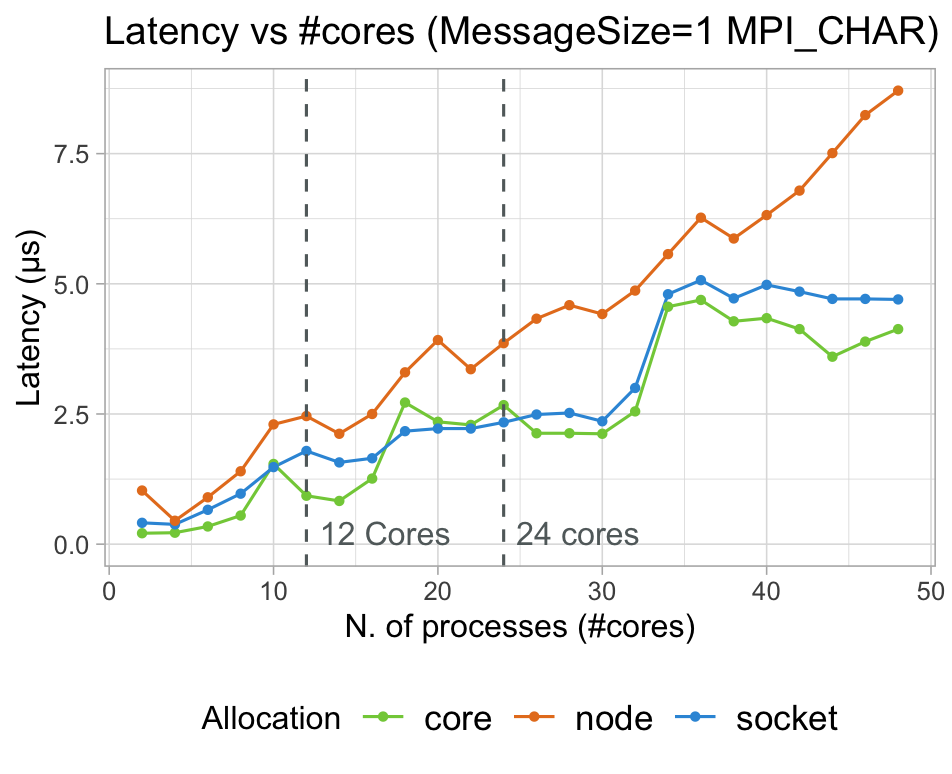
\includegraphics[width=0.32\textwidth]{plots/chain_map.png}\label{plot:chain_map}}
    % \hfill
    \subfigure[Binary Tree algorithm]{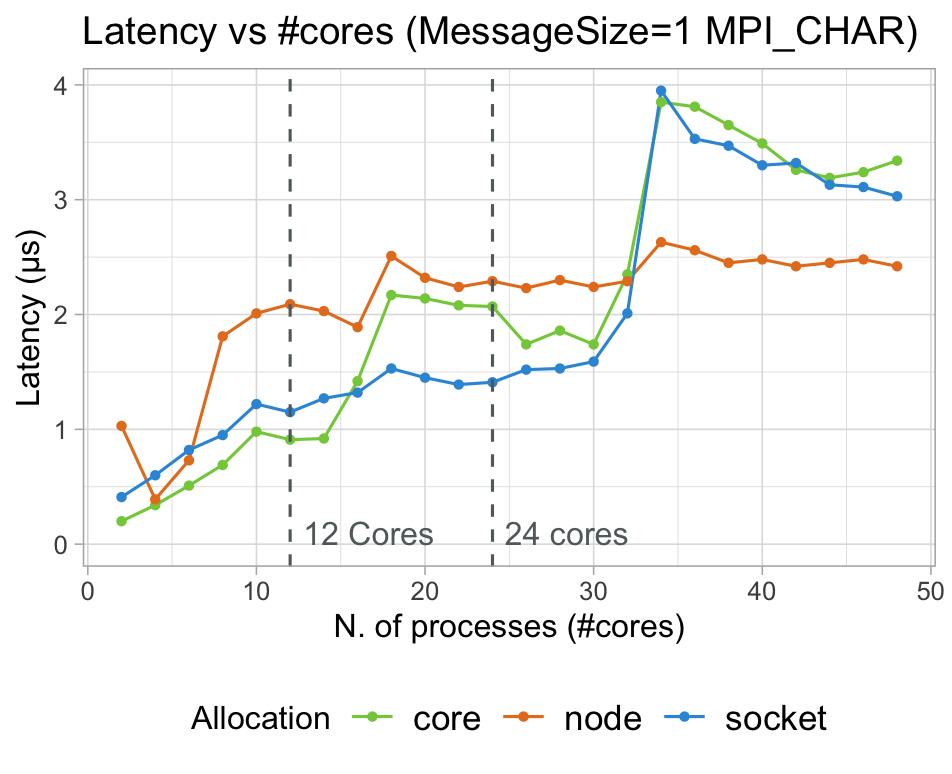
\includegraphics[width=0.32\textwidth]{plots/binarytree_map.png}\label{plot:binarytree_map}}
    % \caption{Analyzed broadcast algorithms}
\end{figure}

Referring to \Cref{plot:linear_map}, the linear algorithm's behavior aligns with expectations. Both socket and core allocations show latency "jumps" when changing nodes, while node allocation progresses seamlessly without noticeable jumps. Similar observations apply to socket changes: core allocation exhibits a jump, whereas socket allocation remains unaffected. An intriguing aspect arises when examining latency jumps. In the \textit{thin} architecture, with sockets of 12 cores and nodes of 24 cores, one might expect jumps at 16 and 32 processes. Surprisingly, jumps occur at 14 and 30 processes, hinting at additional factors influencing communication beyond straightforward node/socket changes.\\[0.3cm]
Transitioning to the chain algorithm (\Cref{plot:chain_map}), there are parallels to our previous considerations. A notable distinction arises when changing node: for the linear case, when the number of processes surpasses 24, the three distinct allocations appear to converge. This convergence aligns with the nature of the linear algorithm, where messages are sent from process 0 to all the others. In particular, when processes span both nodes, the execution steps remain consistent across allocations. For the chain algorithm, on the other hand, the communication among processes follows a precise order, leading to a distinct behavior. When processes are assigned by node, the greater distance traveled by messages becomes evident if compared to allocations by core or socket.\\[0.3cm]
Ultimately, the observations in \Cref{plot:binarytree_map} underscore slower latency values associated with the Binary Tree broadcast, showcasing its (expected) superior performance compared with the two algorithms analyzed above. Allocating processes by node reveals a stable latency profile after 24 cores (node change), indicative of optimized intra-node communication upon reaching a specific depth within the tree structure. When allocating by socket or core, instead, an apparent jump followed by a decrease in latency is observed. This might be attributed to the hierarchical structure of the algorithm: the jump may correspond to the transition between different levels of the tree, introducing a slight delay in communication. Once past this initial transition, the latency decreases as the algorithm progresses through subsequent levels of the tree.


\subsubsection{Fixing processes allocation and compare algorithms}\label{subsubsection:alg}
We fixed the processes allocation by configuring it to \texttt{--map-by core} and we assessed the algorithmic impact on the operation latency. As detailed in \Cref{subsubsection:map}, we ensured the consistency of our analysis by fixing the message size to 1 \texttt{MPI\_CHAR}. Our initial focus is on comparing linear and chain algorithms, as they provide more insightful points of comparison due to their inherent characteristics.

\begin{figure}[htp]
    \centering
    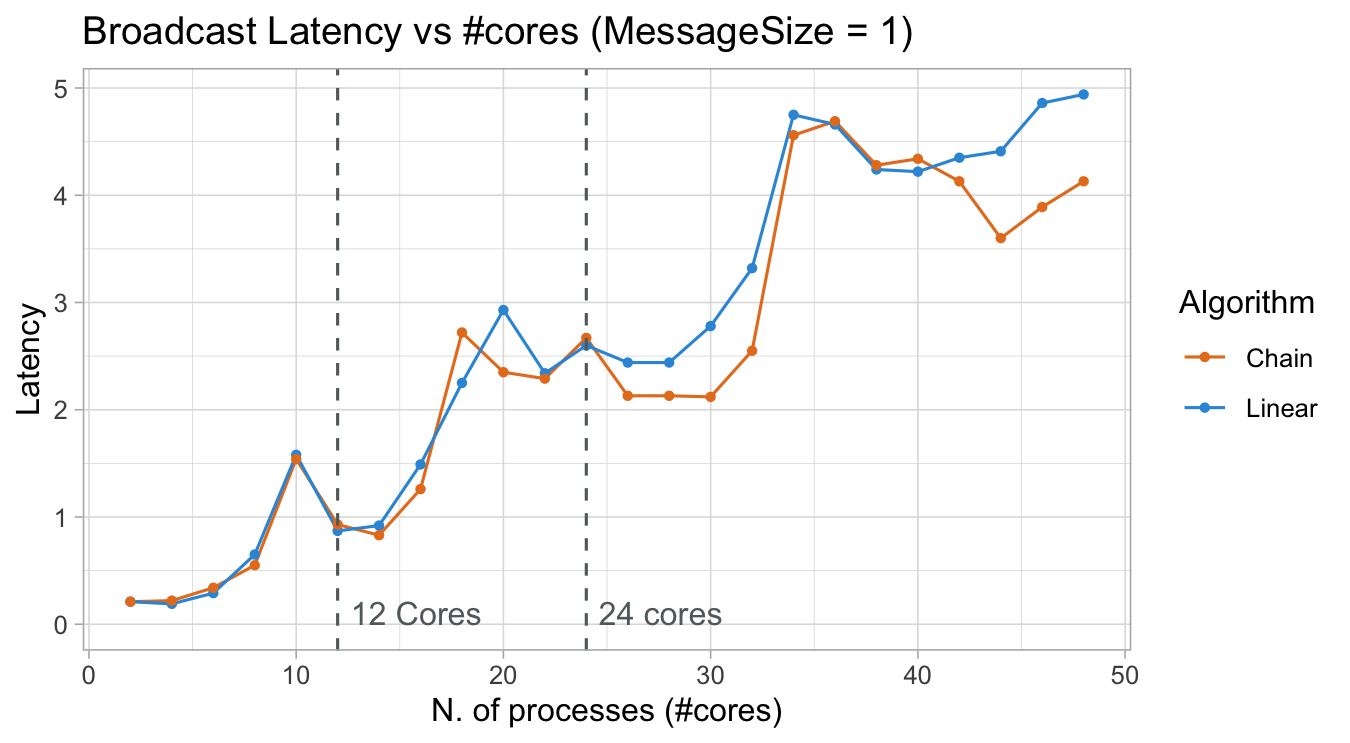
\includegraphics[width=0.5\textwidth]{plots/linear_vs_chain.png}
    \caption{\footnotesize Linear vs Chain comparison}
    \label{plot:linear_vs_chain}
\end{figure}
\Cref{plot:linear_vs_chain} offers some insights into how the algorithm choice influences latency across 3 regions:
\begin{itemize}
    \item \textbf{Region 1 (within socket)}\\
    Both the linear and chain algorithms exhibit nearly identical performance. This suggests that intra-socket communication, occurring between cores within the same socket, is sufficiently fast, and the algorithmic implementation has a minimal impact.
    \item \textbf{Region 2 (within node)}
    As we move to communication within the entire node, a subtle difference emerges, indicating that the choice between chain and linear algorithms might have a more nuanced impact. Despite the slight advantage of the chain algorithm becomes a bit more apparent, the two algorithms still perform quite similarly.
    \item \textbf{Region 3 (outside node)}
    In the external node communication region, where latency is inherently higher, the contrast between chain and linear algorithms becomes more pronounced. This aligns with expectations, as the chain algorithm's utilization of contiguous cores contrasts with the linear algorithm's approach of sending from rank 0 to all other ranks.
\end{itemize}
Conducting similar plots while systematically varying the message size would yield more insightful results, but we will delve into details in \cref{subsubsection:message_size}. As for now, let's keep the message size to 1 \texttt{MPI\_CHAR} and include the default algorithm and the binary tree in our analysis.

\begin{figure}[htp]
    \centering
    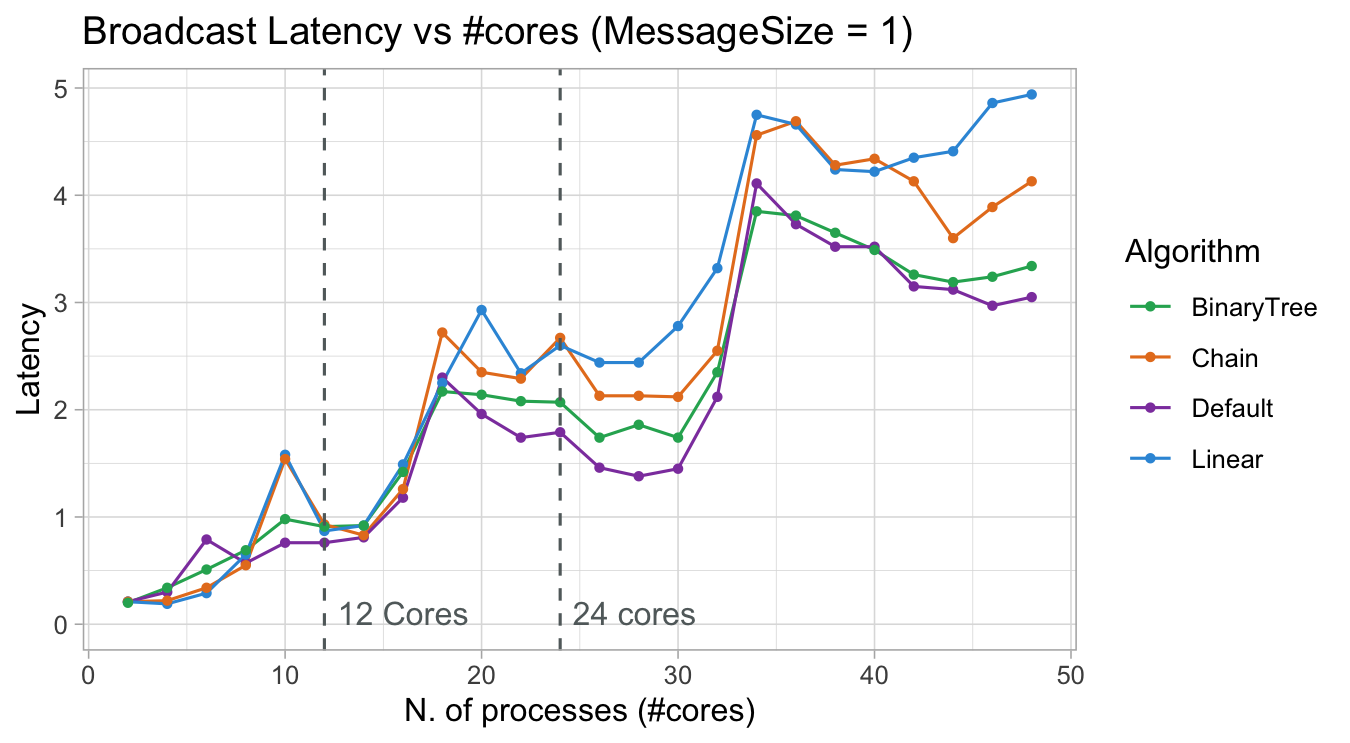
\includegraphics[width=0.5\textwidth]{plots/algs_comparison.png}
    \caption{\footnotesize Broadcast algorithms comparison}
    \label{plot:algs_comparison}
\end{figure}

As observed in earlier sections, the binary tree algorithm consistently exhibits lower latency values. From an algorithmic standpoint, this aligns with expectations, as a tree structure efficiently distributes the communication among its branches, enhancing the overall performance. Ultimately, \Cref{plot:algs_comparison} shows how the default configuration outperforms the other algorithms, emerging as the one with the lowest latency. This was something we also expected: default configurations are often tuned to strike a balance between different use cases, making them robust and efficient in various environments. Additionally, the default settings may leverage platform-specific optimizations, taking advantage of system characteristics to enhance communication efficiency. 

\subsubsection{Fixing processes allocation and compare algorithms for different message sizes}\label{subsubsection:message_size}

As suggested in \Cref{subsubsection:alg} and showed in \Cref{plot:linear_vs_chain_bysize}, increasing the message size may provide a clearer distinction between the algorithms, thus enhancing our understanding of their effectiveness.

\begin{figure}[htp]
    \centering
    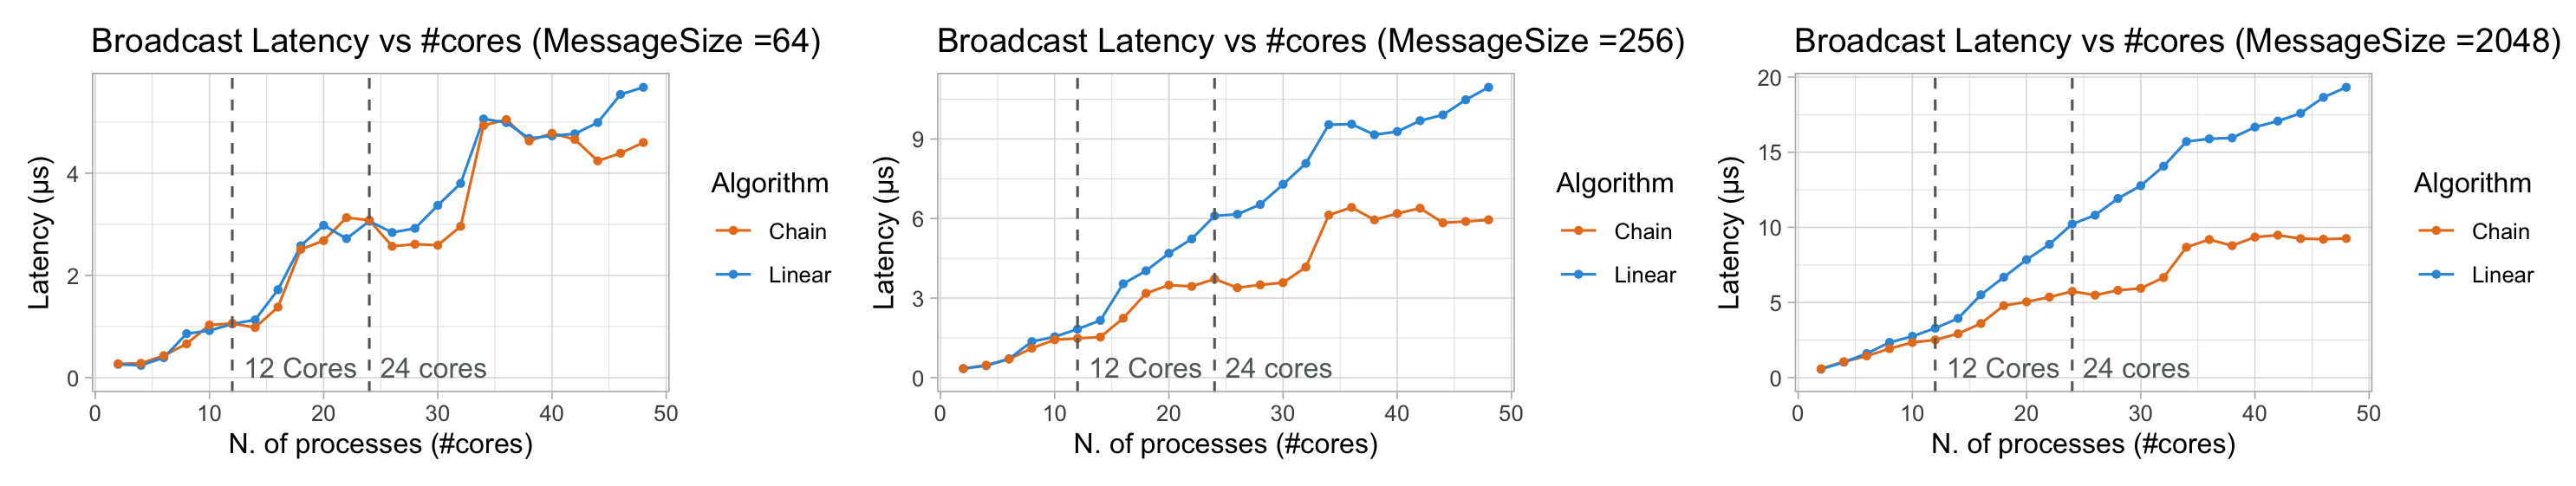
\includegraphics[width=\textwidth]{plots/linear_vs_chain_bysize.png}
    \caption{\footnotesize Linear vs Chain comparison varying message size}
    \label{plot:linear_vs_chain_bysize}
\end{figure}
Chain algorithm exhibits superior performance, primarily attributable to its utilization of contiguous cores. Initially, when the message size was fixed at 1 \texttt{MPI\_CHAR}, the performances of the linear and chain algorithms were nearly indistinguishable. However, as we introduce variations in the message size, the advantages of the chain algorithm become more evident. A critical aspect contributing to its effectiveness is the algorithm's capacity to partition messages into chunks during transmission, a feature absent in the linear broadcast approach (see \cite{NURIYEV20221}). As a consequence, with an increasing message size, the latency of the linear algorithm experiences sharp growth, accentuating the widening performance disparity with respect to the chain algorithm. The direct correlation between message size and communication latency remains consistent for both the binary tree and default algorithms. As shown in \Cref{plot:algs_comparison_bysize}, both the binary tree and default configurations continue to outperform linear and chain algorithms, underscoring their robustness across the increasing message size.
\begin{figure}[htp]
    \centering
    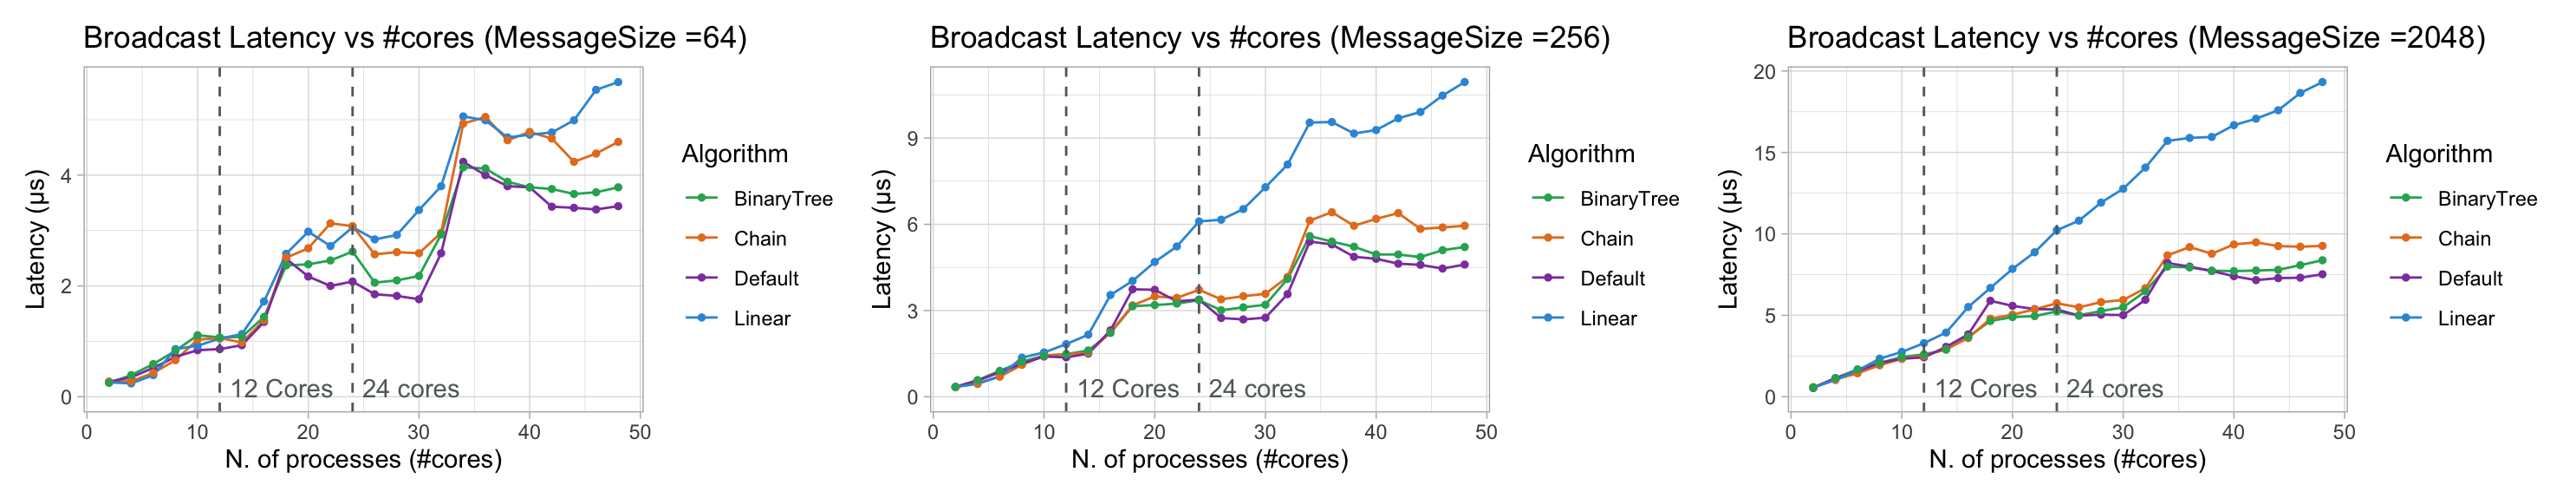
\includegraphics[width=\textwidth]{plots/algs_comparison_bysize.png}
    \caption{\footnotesize Broadcast algorithms comparison varying message size}
    \label{plot:algs_comparison_bysize}
\end{figure}
\subsection{Broadcast performance models}
As a conclusive step of my latency analysis for broadcast communication, I attempted to develop a simple performance model to better understand the intricate dynamics at play. My initial approach involved estimating both latency and bandwidth within point-to-point communication routines, employing the \texttt{OSU} benchmark again (utilizing the \texttt{osu\_latency} tool at the path \url{/osu-micro-benchmarks-7.3/c/mpi/pt2pt/standard.}). The intention was to leverage these estimated values to construct a model resembling the Hockney model I found in literature (see \cite{HockneyOfficial}, \cite{Hockney2}). Unfortunately, the results I obtained did not align well with the collected data, prompting me to explore alternative methodologies.
Guided by my statistical background, I moved towards the implementation of a linear model. 

In selecting predictors for the model, I considered variables such as message size and the number of processes, while I chose to maintain a fixed process allocation using \texttt{--map-by core}. Additionally, due to the inherent characteristics of the problem under investigation, I opted to exclude the intercept from the model (although the latency of a 0-sized message shared among 0 processes is undefined, I assumed it to be 0 for the sake of convention). Furthermore, I constructed separate models for each algorithm, aligning with established practices in the literature where performance models are frequently algorithm-specific.
%---footnote
\footnote{Alternatively, I could treat \textit{Algorithm} as a categorical regressor, with the foresight of incorporating it into an interaction term rather than as a standalone factor. However, it would introduce unnecessary complexity to the model in terms of interpretability and explainability, and I prioritized maintaining clarity and simplicity in the model design.}
%---
Although I derived individual models for each algorithm, it is important to note that they share a common structure, which is the following:
$$\boxed{log_2(\text{Latency}) = \beta_1 \cdot \text{Number of Processes} + \beta_2 \cdot log_2(\text{Message Size})}$$

All the models were built using the software \texttt{R}. \Cref{tab:bcast_summaries} reports, for each of the analyzed algorithms, the estimates for $\beta_0,\beta_1 $ and the $R^2_{adj}$ as a metric to assess the goodness of fit of the associated model.

\begin{table}[h]
    \centering
    \begin{tabular}{|l|c|c|c|}
        \hline
        \textbf{Algorithm} & $\boldsymbol{\beta_1}$ & $\boldsymbol{\beta_2}$ & $\boldsymbol{R^2_{adj}}$\\[0.1cm]
        \hline
        Linear      & 0.029815 & 0.321259 & 88,19 \% \\
        Chain       & 0.021957 & 0.306713 & 86,77 \% \\
        Binary Tree & 0.016315 & 0.317449 & 86,58 \% \\
        Default     & 0.009586 & 0.321418 & 85,86 \% \\
        \hline
    \end{tabular}
    \caption{Broadcast latency models summary}
    \label{tab:bcast_summaries}
\end{table}
% THINK ABOUT INTERPRET COEFF FOR AN ALGORITHM AND COMMENT >=< BTW COEFFICIENTS
%------------------------------------------------------------------------------------
\section{Barrier}
% io qui direi chiaramente che l'approccio generale è stato identico a prima, per cui in questa sezione ci focusseremo più sui risultati che sulla metodologia
\subsection{Barrier algorithms}
% qui parlare degli algoritmi dal punto di vista "teorico"
\subsection{Barrier performance models}
\newpage
%\tableofcontents
\bibliographystyle{unsrt}
\bibliography{bibliography}
\end{document}
